\documentclass[full-course-notes.tex]{subfiles}

\begin{document}
\lecturemeta{3}
  {Lexical Analysis: Tokens, Patterns, and Lexemes; Regular Languages, Regular Expressions,
   and Regular Definitions}
  {CLO 1}
  {\S3.1 (The Role of the Lexical Analyzer), \S3.3 (Specification of Tokens: terminology,
   strings, languages, operations, regular expressions, regular definitions, extensions)}
  {[AP] Modern Compiler Implementation, Ch.\,2; [PP] Programming Language Pragmatics \S3.3}
\lecshort{Lexical Analysis \& Regular Expressions}
\setcounter{section}{0}
\makelecturetitle

\begin{coreidea}[Lecture Roadmap]
\begin{enumerate}
  \item Where lexical analysis sits, and exactly how it talks to the parser; why lexer and
  parser are separate phases.
  \item The three core vocabulary words of this unit: \textbf{token}, \textbf{pattern},
  \textbf{lexeme} -- with several fully worked examples, plus token \textbf{attributes} and
  \textbf{lexical errors}.
  \item \textbf{The big picture}: how a regular expression eventually becomes a working,
  table-driven lexer, via finite automata -- the roadmap for this lecture and the ones after it.
  \item \textbf{Regular languages}, defined formally, and \textbf{regular expressions}, the
  notation we use to name them -- the formal, inductive definition, plus many worked examples.
  \item \textbf{Regular definitions}: naming sub-expressions, culminating in DB's classic
  identifier and numeric-literal definitions.
  \item \textbf{Extensions} (\texttt{+}, \texttt{?}, character classes) -- convenience, not new
  power -- and \textbf{regular vs.\ non-regular languages}: what a lexer's patterns fundamentally
  cannot express.
  \item How real-world lexers extend this model, and how the regular expressions in this
  lecture map directly onto the syntax used by \textbf{Flex}, the lexer-generator tool this
  course uses.
\end{enumerate}
By the end of this lecture you will be able to read and write the formal notation a real lexer
specification is built from -- everything needed before we turn regular expressions into an
actual running program via finite automata.
\end{coreidea}

\section{Where Lexical Analysis Fits}
\label{sec:l3-where-lexical-fits}

\dbtag The \textbf{lexical analyzer} (also called a \textbf{scanner} or \textbf{lexer}) is the
first phase of a compiler. It reads the raw stream of characters making up the source program
and groups them into a stream of \textbf{tokens} --- meaningful chunks like keywords,
identifiers, numbers, and operators --- that the rest of the compiler works with instead of raw
text.

\begin{center}
\begin{tikzpicture}[
  box/.style={draw, thick, rounded corners, minimum height=1.1cm, minimum width=3cm, align=center, font=\small},
  tool/.style={box, fill=dbGreenBg, draw=dbGreen},
  data/.style={box, fill=nuLight, draw=nuNavy},
  >=Latex
]
  \node[data] (src) at (0,0) {Source Program\\(character stream)};
  \node[tool] (lex) at (4.2,0) {Lexical\\Analyzer};
  \node[tool] (parser) at (8.6,0) {Parser};
  \node[data] (st) at (4.2,-2.2) {Symbol Table};

  \draw[->, thick] (src) -- (lex);
  \draw[->, thick] ([yshift=2mm]lex.east) -- node[above, font=\scriptsize]{token} ([yshift=2mm]parser.west);
  \draw[->, thick] ([yshift=-2mm]parser.west) -- node[below, font=\scriptsize]{getNextToken()} ([yshift=-2mm]lex.east);
  \draw[<->, thick, dashed] (lex) -- (st);
\end{tikzpicture}
\end{center}

\begin{coreidea}[How the Lexer and Parser Actually Talk to Each Other]
In nearly every real compiler, the lexer does \emph{not} tokenize the whole file up front and
hand the parser a list. Instead, the parser drives the process: whenever the parser needs another
token, it calls a function conventionally named \texttt{getNextToken()}. The lexer resumes
scanning exactly where it left off, produces the next single token, and returns it. This
``pull'' model, sometimes called treating the lexer as a \textbf{coroutine} of the parser, avoids
ever materializing the full token list in memory and lets the lexer and parser interleave their
work one token at a time.
\end{coreidea}

\subsection{Why Not Just One Phase?}
\label{sec:l3-why-separate}

\dbtag DB gives three concrete engineering reasons for splitting lexical analysis out as its own
phase rather than folding it into the parser:

\begin{enumerate}
  \item \textbf{Simplicity of design.} Separating out low-level tasks (recognizing keywords,
  numbers, string literals) lets the parser work purely with grammatical structure, using
  tokens as its atomic symbols, instead of also worrying about individual characters.
  \item \textbf{Improved efficiency.} Specialized, table-driven techniques for recognizing
  tokens -- built from finite automata, which the lectures right after this one construct
  \emph{directly} from the regular expressions we develop later in this very lecture -- are
  considerably faster than the general-purpose parsing techniques would be if forced to operate
  character-by-character.
  \item \textbf{Enhanced portability.} Input-device and operating-system-specific quirks ---
  end-of-line conventions (\texttt{\textbackslash n} vs.\ \texttt{\textbackslash r\textbackslash n}), character
  encodings, special end-of-file characters --- are confined entirely to the lexer. The parser,
  and everything after it, is completely insulated from these differences.
\end{enumerate}

\begin{examfocus}
This ``three reasons'' list (simplicity, efficiency, portability) is a favorite short-answer
question. Be able to name and briefly justify all three, not just one.
\end{examfocus}

\section{Tokens, Patterns, and Lexemes}
\label{sec:l3-tokens-patterns-lexemes}

\dbtag These three terms are used precisely and are easy to blur together. Getting the
distinction exactly right is one of the most exam-tested ideas in this entire unit.

\begin{defbox}{Token, Pattern, Lexeme}
\begin{itemize}
  \item A \textbf{token} is a pair \texttt{<token-name, attribute-value>} representing a
  \emph{category} of lexical unit, e.g.\ \texttt{ID}, \texttt{NUM}, \texttt{RELOP}. The
  token-name is an abstract symbol used by the parser.
  \item A \textbf{pattern} is the rule that describes the \emph{set of possible lexemes} that
  can produce a given token -- for identifiers, informally, ``a letter followed by any number of
  letters and digits.'' \Sref{sec:l4-regular-expressions}, later in this lecture, makes patterns
  precise using regular expressions.
  \item A \textbf{lexeme} is the actual sequence of characters in the source program that
  \emph{matches} a pattern and is classified as an instance of some token.
\end{itemize}
\end{defbox}

\begin{center}
\begin{tikzpicture}[
  box/.style={draw, thick, rounded corners, minimum height=1cm, minimum width=3.1cm, align=center, font=\small},
  >=Latex
]
  \node[box, fill=nuLight, draw=nuNavy] (chars) at (0,0) {Source\\Characters};
  \node[box, fill=enrichGoldBg, draw=enrichGold] (pat) at (4,0) {matched against\\a \textbf{Pattern}};
  \node[box, fill=dbGreenBg, draw=dbGreen] (lex) at (8,0) {yields a\\\textbf{Lexeme}};
  \node[box, fill=examRedBg, draw=examRed] (tok) at (12,0) {emits a\\\textbf{Token}\\\texttt{<name, attr>}};
  \draw[->, thick] (chars) -- (pat);
  \draw[->, thick] (pat) -- (lex);
  \draw[->, thick] (lex) -- (tok);
\end{tikzpicture}
\end{center}

\begin{examplebox}{DB-Style Token/Pattern/Lexeme Table}
\renewcommand{\arraystretch}{1.3}
\begin{tabularx}{\textwidth}{@{}l X l@{}}
\toprule
\textbf{Token} & \textbf{Informal Description of Pattern} & \textbf{Sample Lexemes} \\
\midrule
\texttt{WHILE} & the exact keyword \texttt{while} & \texttt{while} \\
\texttt{ID} & a letter, followed by any number of letters or digits & \texttt{i}, \texttt{sum}, \texttt{score2} \\
\texttt{NUM} & any numeric constant & \texttt{0}, \texttt{42}, \texttt{3.14} \\
\texttt{RELOP} & \texttt{<}, \texttt{<=}, \texttt{=}, \texttt{<>}, \texttt{>}, or \texttt{>=} & \texttt{<=}, \texttt{<>} \\
\texttt{LITERAL} & any characters between a pair of double quotes, except a double quote itself & \texttt{"Total = "} \\
\bottomrule
\end{tabularx}
\end{examplebox}

\subsection{Worked Example 1: Tokenizing a Function Call}
\label{sec:l3-worked-example-1}

Consider the following line of C-like source code:

\begin{center}
\ttfamily\large
\colorbox{dbGreenBg}{printf}\colorbox{examRedBg}{(}\colorbox{enrichGoldBg}{"Total = \%d\textbackslash n"}\colorbox{examRedBg}{,}\ \colorbox{dbGreenBg}{score}\colorbox{examRedBg}{)}\colorbox{examRedBg}{;}
\end{center}
\begin{center}
\small\begin{tabular}{@{}p{2.6cm}p{2.6cm}p{2.6cm}p{2.6cm}@{}}
\colorbox{dbGreenBg}{\phantom{x}}\ identifier &
\colorbox{examRedBg}{\phantom{x}}\ punctuation/operator &
\colorbox{enrichGoldBg}{\phantom{x}}\ string literal &
\end{tabular}
\end{center}

\begin{center}
\renewcommand{\arraystretch}{1.25}
\begin{tabularx}{\textwidth}{@{}l l X@{}}
\toprule
\textbf{Lexeme} & \textbf{Token Name} & \textbf{Attribute-Value (passed to parser)} \\
\midrule
\texttt{printf} & \texttt{ID} & pointer to symbol-table entry for \texttt{printf} \\
\texttt{(} & \texttt{LPAREN} & none needed \\
\texttt{"Total = \%d\textbackslash n"} & \texttt{LITERAL} & pointer to the string's stored value \\
\texttt{,} & \texttt{COMMA} & none needed \\
\texttt{score} & \texttt{ID} & pointer to symbol-table entry for \texttt{score} \\
\texttt{)} & \texttt{RPAREN} & none needed \\
\texttt{;} & \texttt{SEMI} & none needed \\
\bottomrule
\end{tabularx}
\end{center}

\section{Attributes for Tokens}
\label{sec:l3-attributes}

\dbtag When more than one lexeme can match a token's pattern (as with \texttt{ID} or
\texttt{NUM}), the lexer must pass along enough extra information -- the \textbf{attribute-value}
-- for later phases to know exactly \emph{which} identifier or \emph{which} number was matched.
For identifiers, this is essentially always a pointer into the symbol table.

\begin{examplebox}{Worked Example 2: An Assignment Statement}
Source line: \quad \texttt{E = M * C ** 2}

Assume \texttt{**} is this language's exponentiation operator. The lexer's output, as a stream
of \texttt{<token-name, attribute-value>} pairs, is:
\begin{center}
\ttfamily
\begin{tabular}{@{}l@{}}
\ttfamily <ID, ptr to symtab entry for E> \\
<ASSIGN\_OP,\ -- >  \\
<ID, ptr to symtab entry for M> \\
<MULT\_OP,\ -- > \\
<ID, ptr to symtab entry for C> \\
<EXP\_OP,\ -- > \\
<NUM, integer value 2>
\end{tabular}
\end{center}
Notice: \texttt{ID} tokens all carry a symbol-table pointer as their attribute so that later
phases can distinguish \texttt{E} from \texttt{M} from \texttt{C}; the operator tokens need no
attribute at all, since the token-name alone (\texttt{ASSIGN\_OP} vs.\ \texttt{MULT\_OP}) already
says everything the parser needs to know.
\end{examplebox}

\begin{examfocus}
Given a short program line, be able to produce the exact stream of
\texttt{<token-name, attribute-value>} pairs, in order, the way both worked examples above do.
This is the single most common long-answer question style for this unit.
\end{examfocus}

\subsection{Worked Example 3: A Complete Statement Block}
\label{sec:l3-worked-example-3}

\begin{center}
\begin{minipage}{0.5\textwidth}
\ttfamily
int sum = 0;\\
while (i <= 10) \{\\
\ \ sum = sum + i;\\
\ \ i = i + 1;\\
\}
\end{minipage}
\end{center}

\begin{center}
\renewcommand{\arraystretch}{1.15}
\footnotesize
\begin{tabularx}{\textwidth}{@{}l l X | l l X@{}}
\toprule
\textbf{Lexeme} & \textbf{Token} & \textbf{Attribute} & \textbf{Lexeme} & \textbf{Token} & \textbf{Attribute} \\
\midrule
\texttt{int} & \texttt{TYPE} & -- & \texttt{sum} & \texttt{ID} & ptr(\texttt{sum}) \\
\texttt{sum} & \texttt{ID} & ptr(\texttt{sum}) & \texttt{=} & \texttt{ASSIGN} & -- \\
\texttt{=} & \texttt{ASSIGN} & -- & \texttt{sum} & \texttt{ID} & ptr(\texttt{sum}) \\
\texttt{0} & \texttt{NUM} & 0 & \texttt{+} & \texttt{PLUS} & -- \\
\texttt{;} & \texttt{SEMI} & -- & \texttt{i} & \texttt{ID} & ptr(\texttt{i}) \\
\texttt{while} & \texttt{WHILE} & -- & \texttt{;} & \texttt{SEMI} & -- \\
\texttt{(} & \texttt{LPAREN} & -- & \texttt{i} & \texttt{ID} & ptr(\texttt{i}) \\
\texttt{i} & \texttt{ID} & ptr(\texttt{i}) & \texttt{=} & \texttt{ASSIGN} & -- \\
\texttt{<=} & \texttt{RELOP} & LE & \texttt{i} & \texttt{ID} & ptr(\texttt{i}) \\
\texttt{10} & \texttt{NUM} & 10 & \texttt{+} & \texttt{PLUS} & -- \\
\texttt{)} & \texttt{RPAREN} & -- & \texttt{1} & \texttt{NUM} & 1 \\
\texttt{\{} & \texttt{LBRACE} & -- & \texttt{;} & \texttt{SEMI} & -- \\
 & & & \texttt{\}} & \texttt{RBRACE} & -- \\
\bottomrule
\end{tabularx}
\end{center}

Two details worth noticing in this longer example:
\begin{itemize}
  \item \texttt{sum} and \texttt{i} each get \emph{their own} symbol-table pointer the first
  time they're seen, and the \emph{same} pointer every time they reappear -- the symbol table
  guarantees one entry per distinct identifier, no matter how many times it's used.
  \item Whitespace (the spaces and newlines between tokens) and indentation produce \emph{no}
  tokens at all -- they are consumed and discarded by the lexer, along with any comments, before
  the parser ever sees anything.
\end{itemize}

\begin{coreidea}[The Lexer's ``Housekeeping'' Duties]
Beyond producing tokens, DB notes the lexer is also the natural place to: strip out whitespace
and comments (neither produces a token); and track line numbers (and often column numbers) so
that later phases can report errors with accurate source locations, e.g.\ ``\texttt{undeclared
variable `x' at line 42}.''
\end{coreidea}

\section{Lexical Errors}
\label{sec:l3-lexical-errors}

\dbtag It is surprisingly rare for a lexer to be able to detect an error entirely on its own,
\emph{by itself, in isolation} -- because almost any short character sequence is a \emph{prefix}
of some valid lexeme for some token.

\begin{examplebox}{The Classic Illustration}
Consider the fragment \texttt{fi (a == f(x))} in a C-like language, where the programmer
\emph{meant} to type the keyword \texttt{if}. The lexer cannot know this. \texttt{fi} is a
perfectly legal lexeme for token \texttt{ID} (``a letter followed by letters/digits''), so the
lexer happily emits \texttt{<ID, ptr(fi)>}. The mistake will only be caught later -- by the
\emph{parser}, if \texttt{fi} appears somewhere no identifier is grammatically valid, or by
\emph{semantic analysis}, if \texttt{fi} is used as if it were a function without ever having
been declared.
\end{examplebox}

Genuine lexical errors are ones where \emph{no pattern for any token} can match the remaining
input at all, or where a token's own internal structure is malformed:

\begin{itemize}
  \item An illegal character that starts no valid token in the language, e.g.\ a stray
  \texttt{\#} or \texttt{@} in a language that assigns those characters no meaning.
  \item An unterminated string literal: opening quote seen, but the line (or file) ends before a
  matching closing quote.
  \item A malformed numeric literal, e.g.\ \texttt{3.14.15} (two decimal points), or
  \texttt{2r} immediately followed by a letter with no valid meaning in that position.
  \item An unterminated comment: a \texttt{/*} seen with no matching \texttt{*/} anywhere before
  end of file.
\end{itemize}

\subsection{Error Recovery Strategies}
\label{sec:l3-error-recovery}

\dbtag A production-quality lexer does not simply stop at the first error --- it tries to
recover and keep going, so the programmer can see \emph{several} distinct errors from one
compilation attempt rather than fixing them one at a time.

\begin{center}
\begin{tikzpicture}[
  box/.style={draw, thick, rounded corners, minimum height=0.9cm, minimum width=3.6cm, align=center, font=\small},
  dec/.style={draw, thick, diamond, aspect=2.4, minimum width=3.4cm, minimum height=1.4cm, align=center, font=\small, fill=nuLight, draw=nuNavy},
  >=Latex
]
  \node[box, fill=nuLight, draw=nuNavy] (start) at (0,0) {Read next\\characters};
  \node[dec] (match) at (0,-2.1) {Matches some\\token's pattern?};
  \node[box, fill=dbGreenBg, draw=dbGreen] (emit) at (5,-2.1) {Emit token,\\advance input};
  \node[box, fill=examRedBg, draw=examRed] (err) at (0,-4.6) {Report lexical\\error};
  \node[box, fill=enrichGoldBg, draw=enrichGold] (panic) at (0,-6.6) {Panic-mode: delete\\char(s) until a valid\\token can resume};

  \draw[->, thick] (start) -- (match);
  \draw[->, thick] (match) -- node[above, font=\scriptsize]{yes} (emit);
  \draw[->, thick] (match) -- node[left, font=\scriptsize]{no} (err);
  \draw[->, thick] (err) -- (panic);
  \draw[->, thick] (emit.north) to[out=90,in=0] (start.east);
  \draw[->, thick] (panic.west) to[out=180,in=270] (start.south);
\end{tikzpicture}
\end{center}

\dbtag DB lists several concrete local-correction strategies a recovering lexer can attempt,
beyond plain panic mode:

\begin{itemize}
  \item \textbf{Deleting} an extraneous character.
  \item \textbf{Inserting} a missing character.
  \item \textbf{Replacing} one incorrect character with a correct one.
  \item \textbf{Transposing} two adjacent characters.
\end{itemize}

\begin{historynote}
DB points toward a more principled version of this idea: choosing whichever single correction
requires the \emph{fewest} character edits -- insertions, deletions, substitutions -- to turn
the bad input into something valid. This is exactly \textbf{edit distance} (Levenshtein
distance), the same string-similarity measure used today in spell-checkers and DNA sequence
alignment. Aho and Peterson described a minimum-distance error-correcting parser as early as
1972; the idea that ``the best fix is the cheapest fix'' turns out to generalize far beyond
lexical analysis, into syntax error recovery and even runtime auto-correct systems.
\end{historynote}

\begin{examfocus}
Be able to explain, with a concrete example like \texttt{fi (a == f(x))}, \emph{why} a
misspelled keyword is usually \textbf{not} a lexical error even though it looks like an obvious
typo. Then be able to list at least two genuine, purely lexical errors (unterminated string,
illegal character) and describe panic-mode recovery in one sentence.
\end{examfocus}

\section{The Big Picture: From Regular Expressions to a Working Lexer}
\label{sec:l3-big-picture}

\dbtag Every pattern we have used so far has been informal English: ``a letter followed by
letters or digits.'' That is fine for talking about lexical analysis, but it is not something a
computer can execute. Turning informal patterns into an actual running lexer takes a short
pipeline of well-defined, \emph{mechanical} steps, and it is worth seeing the whole pipeline
once, up front, before building any one piece of it.

\begin{center}
\resizebox{\textwidth}{!}{%
\begin{tikzpicture}[
  box/.style={draw, thick, rounded corners, minimum height=1.1cm, minimum width=2.7cm, align=center, font=\small},
  re/.style={box, fill=examRedBg, draw=examRed},
  nfa/.style={box, fill=enrichGoldBg, draw=enrichGold},
  dfa/.style={box, fill=dbGreenBg, draw=dbGreen},
  tab/.style={box, fill=nuLight, draw=nuNavy},
  >=Latex
]
  \node[re]  (re)    at (0,0)    {Regular\\Expression};
  \node[nfa] (nfa)   at (4.6,0)  {NFA};
  \node[dfa] (dfa)   at (9.2,0)  {DFA};
  \node[dfa] (mdfa)  at (13.8,0) {Minimized\\DFA};
  \node[tab] (table) at (18.4,0) {Transition\\Table /\\Diagram};
  \node[tab] (lexer) at (18.4,-2.6) {Table-Driven\\Lexer};

  \draw[->, thick] (re) -- node[above, font=\scriptsize, align=center]{Thompson's\\Construction} (nfa);
  \draw[->, thick] (nfa) -- node[above, font=\scriptsize, align=center]{Subset\\Construction} (dfa);
  \draw[->, thick] (dfa) -- node[above, font=\scriptsize, align=center]{Minimization} (mdfa);
  \draw[->, thick] (mdfa) -- node[above, font=\scriptsize, align=center]{Table\\Encoding} (table);
  \draw[->, thick] (table) -- (lexer);
  \draw[->, thick, dashed, black!55] (re.south) to[out=-55, in=235]
    node[below=3pt, font=\scriptsize, align=center, text=black!55]
    {\textbf{Shortcut:} direct DFA construction\\(skips the NFA step entirely)} (dfa.south);
\end{tikzpicture}}
\end{center}

\begin{center}
\renewcommand{\arraystretch}{1.35}
\begin{tabularx}{\textwidth}{@{}l X@{}}
\toprule
\textbf{Step} & \textbf{What Happens} \\
\midrule
Regular expression $\to$ NFA & \textbf{Thompson's construction}: a purely mechanical algorithm
that builds a nondeterministic finite automaton (NFA) directly from the structure of a regular
expression, one small automaton per operator. \\
NFA $\to$ DFA & \textbf{Subset construction}: another mechanical algorithm that converts any NFA
into an equivalent deterministic finite automaton (DFA) -- one with no ambiguity about which
transition to take, at the cost of (possibly) more states. \\
\emph{(shortcut)} Regular expression $\to$ DFA directly & Some tools skip the NFA step
entirely: DB \S3.9 builds a DFA \emph{directly} from a regular expression's syntax tree, using
functions traditionally called \textit{nullable}, \textit{firstpos}, \textit{lastpos}, and
\textit{followpos}. It computes exactly the same DFA that Thompson's construction plus subset
construction would have produced (possibly needing a separate minimization pass afterward) --
it is a different \emph{route} to the same destination, not a different destination, and it is
what many real lexer generators use internally because it tends to build fewer intermediate
states. \\
DFA $\to$ minimized DFA & \textbf{DFA minimization}: merges states that are behaviorally
indistinguishable, producing the smallest possible DFA that still recognizes exactly the same
language. \\
Minimized DFA $\to$ transition table & The (finite!) set of states and transitions is encoded
as a 2-D table: \texttt{table[state][input\_symbol] = next\_state}. \\
Transition table $\to$ lexer & A tiny, fast loop -- look up the current state and next
character in the table, move to the next state, repeat -- \emph{is} the lexer's inner loop. No
more cleverness is needed once the table exists. \\
\bottomrule
\end{tabularx}
\end{center}

\begin{examfocus}
``Transition diagram'' and ``transition table'' are not two different stages of this pipeline --
they are two different \emph{representations of the same DFA (or NFA)}. A \textbf{transition
diagram} is the picture: circles for states, labeled arrows for transitions, exactly the
automaton drawings you will see in the next few lectures. A \textbf{transition table} is the
same information laid out as a 2-D array instead of a picture. Neither one is more ``correct''
than the other, and neither is a separate construction step -- once you have a DFA, you already
have both, you have just chosen how to write it down. A common exam trap asks you to convert
between the two for a small automaton; that is a notation exercise, not a new algorithm.
\end{examfocus}

\begin{coreidea}[Why This Pipeline Matters]
Every solid arrow in the diagram above is a \emph{mechanical, automatable} algorithm -- none of
them require human judgment once the previous step is done, and the dashed shortcut is simply
an alternative route to the same DFA. This is exactly why lexer-generator tools like Flex exist:
you write only the left-most box (a set of regular expressions, one per token), and the tool
runs the entire rest of the pipeline for you, emitting ready-to-compile scanner code. The
remaining lectures on lexical analysis build this pipeline one arrow at a time -- Thompson's
construction and subset construction first, then minimization -- so that by the time we reach
Flex itself, you understand exactly what the tool is doing on your behalf rather than treating
it as a black box.
\end{coreidea}

\section{Strings, Alphabets, and Languages}
\label{sec:l4-strings-alphabets-languages}

\dbtag Before regular expressions can be defined precisely, three primitive terms need to be
pinned down exactly as DB uses them.

\begin{defbox}{Alphabet, String, Language}
\begin{itemize}
  \item An \textbf{alphabet} $\Sigma$ is any finite set of symbols, e.g.\ $\{0,1\}$ or the set
  of ASCII characters.
  \item A \textbf{string} (or \emph{word}) over $\Sigma$ is a finite sequence of symbols drawn
  from $\Sigma$. The \textbf{empty string}, written $\varepsilon$, has length 0.
  \item A \textbf{language} over $\Sigma$ is simply \emph{any} set of strings over $\Sigma$ ---
  possibly infinite, possibly empty ($\emptyset$, the language with no strings at all, which is
  \emph{not} the same as $\{\varepsilon\}$, the language containing only the empty string).
\end{itemize}
\end{defbox}

\begin{examfocus}
$\emptyset$ and $\{\varepsilon\}$ are a classic confusion. $\emptyset$ contains \emph{zero}
strings; $\{\varepsilon\}$ contains \emph{one} string (the empty one). Keep them distinct.
\end{examfocus}

\begin{coreidea}[Formal Languages: A Hierarchy, Not One Thing]
The definition above -- ``a language is any set of strings'' -- deliberately puts \emph{no}
restriction on what that set looks like. A set meeting only this bare definition is often
called a \textbf{formal language}, precisely to flag that nothing about its internal structure
is assumed yet. Computer science studies several increasingly restrictive (and increasingly
cheap to process) \emph{classes} of formal languages, most famously organized into the
\textbf{Chomsky hierarchy}:
\begin{center}
\small
\renewcommand{\arraystretch}{1.3}
\begin{tabularx}{\textwidth}{@{}l X@{}}
\toprule
\textbf{Class} & \textbf{Recognized by} \\
\midrule
Regular languages & Finite automata -- \textbf{this lecture's topic}, used for tokens \\
Context-free languages & Pushdown automata (a finite automaton plus a stack) -- used for
parsing, covered once this course reaches syntax analysis \\
Context-sensitive / recursively enumerable & Increasingly powerful machines (linear-bounded
automata, full Turing machines) -- outside the scope of this course \\
\bottomrule
\end{tabularx}
\end{center}
Each class in this list \emph{properly contains} the one above it: every regular language is
also context-free, but not the reverse -- balanced parentheses
(\Sref{sec:l4-regular-vs-nonregular}) is the standard example of a language that is context-free
but \emph{not} regular. This containment is exactly why a parser (built on context-free
grammars) can express everything a lexer's regular expressions can, and more. This lecture
defines exactly one of these classes with full precision -- the \textbf{regular languages},
starting in \Sref{sec:l3-regular-languages-formal} below.
\end{coreidea}

\section{Regular Languages: A Formal Definition}
\label{sec:l3-regular-languages-formal}

\dbtag To say precisely which languages qualify as ``regular,'' we first need a small set of
operations for building new languages out of old ones. Given two languages $L$ and $M$ over the
same alphabet, DB defines four such operations:

\begin{center}
\renewcommand{\arraystretch}{1.35}
\begin{tabularx}{\textwidth}{@{}l l X@{}}
\toprule
\textbf{Operation} & \textbf{Notation} & \textbf{Definition} \\
\midrule
Union & $L \cup M$ & $\{\, s \mid s \in L \text{ or } s \in M \,\}$ \\
Concatenation & $LM$ & $\{\, st \mid s \in L \text{ and } t \in M \,\}$ (paste a string from $L$
directly onto a string from $M$) \\
Kleene closure & $L^{*}$ & $\bigcup_{i=0}^{\infty} L^{i}$ -- zero or more strings from $L$,
concatenated (includes $\varepsilon$, from $L^0$) \\
Positive closure & $L^{+}$ & $\bigcup_{i=1}^{\infty} L^{i}$ -- one or more strings from $L$,
concatenated (excludes $\varepsilon$ unless $\varepsilon \in L$) \\
\bottomrule
\end{tabularx}
\end{center}

\begin{examplebox}{Worked Example: Letters and Digits}
Let $L = \{a, b, c, \dots, z, A, \dots, Z\}$ (the 52 letters) and $D = \{0, 1, \dots, 9\}$ (the
10 digits), each treated as a language of one-character strings.
\begin{itemize}
  \item $L \cup D$ -- every single letter \emph{or} single digit: 62 strings, each of length 1.
  \item $LD$ -- every string formed by one letter followed by one digit, e.g.\ \texttt{a5},
  \texttt{Z0} -- exactly $52 \times 10 = 520$ strings, each of length 2.
  \item $L^{4}$ -- every string of exactly 4 letters, e.g.\ \texttt{Test}, \texttt{abcd} --
  there are $52^{4}$ such strings in total.
  \item $L^{*}$ -- every string of letters of \emph{any} length, including $\varepsilon$ ---
  infinitely many strings.
  \item $L(L \cup D)^{*}$ -- one letter, followed by zero or more letters-or-digits. This is
  \emph{exactly} the language of identifiers in most C-like languages! We will turn this
  directly into a regular expression in \Sref{sec:l4-regular-expressions}.
\end{itemize}
\end{examplebox}

\dbtag With these operations in hand, we can now say precisely what ``regular'' means -- a
statement about the language itself, as a set of strings, before we ever write a single regular
expression on paper.

\begin{defbox}{Regular Language (Inductive Definition)}
The \textbf{regular languages} over an alphabet $\Sigma$ are defined inductively, using exactly
the union, concatenation, and Kleene-closure operations above:
\begin{itemize}
  \item \textbf{Base cases:} $\emptyset$ is a regular language; $\{\varepsilon\}$ is a regular
  language; $\{a\}$ is a regular language for every symbol $a \in \Sigma$.
  \item \textbf{Inductive cases:} if $L$ and $M$ are regular languages, then so are
  $L \cup M$ (their union), $LM$ (their concatenation), and $L^{*}$ (the Kleene closure of $L$).
  \item \textbf{Nothing else} is a regular language -- the regular languages are exactly the
  languages reachable by finitely many applications of the rules above, starting from the base
  cases.
\end{itemize}
\end{defbox}

This definition tells us \emph{which} languages count as regular. It does \emph{not}, by
itself, give us a convenient way to write such a language down on paper or in code -- and that
gap is exactly what a regular expression fills.

\begin{coreidea}[Regular Language vs.\ Regular Expression]
A \textbf{regular language} is a set of strings satisfying the definition above -- a semantic
object, a mathematical fact about which strings belong to it. A \textbf{regular expression}
(defined next) is a piece of \emph{syntax}: a compact, human-writable notation for naming one
specific regular language. Every regular expression denotes exactly one regular language, and
--- a real theorem, proved properly in your Automata Theory course --- every regular language
can be named by at least one regular expression. The two notions therefore describe exactly the
same class of languages, but they are conceptually different: one is a fact about a language,
the other is a way of writing it down.
\end{coreidea}

\begin{examfocus}
``Is this a regular language?'' and ``is this a valid regular expression?'' are different
questions, and exam wording sometimes blurs them on purpose. A language can be regular even if
you haven't yet written down a regular expression for it (you just haven't found the notation
yet); conversely, every string of regex syntax that type-checks against the inductive definition
in \Sref{sec:l4-regular-expressions} denotes \emph{some} regular language, whether or not that
language is a useful one.
\end{examfocus}

\section{Regular Expressions}
\label{sec:l4-regular-expressions}

\dbtag A \textbf{regular expression} is a compact notation for describing a language. DB
defines regular expressions \emph{inductively}: a small set of base cases, plus rules for
combining smaller regular expressions into bigger ones -- deliberately mirroring, symbol for
symbol, the definition of the regular languages themselves from
\Sref{sec:l3-regular-languages-formal}.

\begin{defbox}{Regular Expressions (Inductive Definition)}
Over alphabet $\Sigma$:
\begin{itemize}
  \item \textbf{Base case 1:} $\varepsilon$ is a regular expression; $L(\varepsilon) = \{\varepsilon\}$.
  \item \textbf{Base case 2:} for each symbol $a \in \Sigma$, $a$ is a regular expression;
  $L(a) = \{a\}$.
  \item \textbf{Inductive case (union):} if $r$ and $s$ are regular expressions, so is
  $r \mid s$, with $L(r \mid s) = L(r) \cup L(s)$.
  \item \textbf{Inductive case (concatenation):} if $r$ and $s$ are regular expressions, so is
  $rs$, with $L(rs) = L(r)L(s)$.
  \item \textbf{Inductive case (closure):} if $r$ is a regular expression, so is $r^{*}$, with
  $L(r^{*}) = (L(r))^{*}$.
  \item \textbf{Parenthesization:} if $r$ is a regular expression, so is $(r)$, with
  $L((r)) = L(r)$ -- used purely to control grouping/precedence.
\end{itemize}
Here $L(r)$ denotes ``the regular language named by regular expression $r$'' -- notice every
base case and inductive case above produces a regular language in exactly the sense of
\Sref{sec:l3-regular-languages-formal}, and nothing else, matching that definition rule for
rule.
\end{defbox}

\begin{coreidea}[Operator Precedence]
When parentheses are omitted, DB fixes a precedence, highest to lowest: \textbf{closure}
($^{*}$) binds tightest, then \textbf{concatenation}, then \textbf{union} ($\mid$) binds
loosest. So $ab \mid c$ means $(ab)\mid c$, \emph{not} $a(b\mid c)$; and $a\mid bc^{*}$ means
$a \mid (b(c^{*}))$.
\end{coreidea}

\subsection{Worked Example: Building Up a Regular Expression}
\label{sec:l4-worked-example-build-up}

DB's running example: the language of all strings of \texttt{a}'s and \texttt{b}'s that
\emph{end in} \texttt{abb}. Let's build the regular expression piece by piece.

\begin{center}
\renewcommand{\arraystretch}{1.3}
\begin{tabularx}{\textwidth}{@{}l X@{}}
\toprule
\textbf{Sub-expression} & \textbf{What it describes} \\
\midrule
$a \mid b$ & a single \texttt{a} \emph{or} a single \texttt{b} \\
$(a \mid b)^{*}$ & \emph{any} string of \texttt{a}'s and \texttt{b}'s (including $\varepsilon$) \\
$(a \mid b)^{*}abb$ & any string of \texttt{a}'s and \texttt{b}'s, \textbf{followed by} the
literal suffix \texttt{abb} -- i.e.\ exactly the strings that \emph{end in} \texttt{abb} \\
\bottomrule
\end{tabularx}
\end{center}

\begin{center}
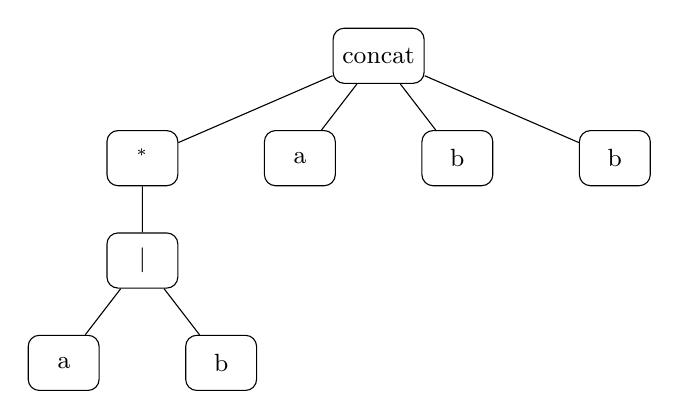
\begin{tikzpicture}[
  level distance=13mm,
  sibling distance=20mm,
  every node/.style={draw, rounded corners, minimum width=9mm, minimum height=7mm, align=center, font=\small}
]
\node {concat}
  child { node {$^{*}$}
    child { node {$\mid$}
      child { node {a} }
      child { node {b} }
    }
  }
  child { node {a} }
  child { node {b} }
  child { node {b} }
;
\end{tikzpicture}
\end{center}
\begin{center}
\small\textit{Syntax tree for $(a\mid b)^{*}abb$: the root concatenates four pieces --- the
starred union, then three literal symbols.}
\end{center}

\begin{examplebox}{Trace: Does \texttt{"babb"} Match?}
\texttt{babb} = \texttt{b} (matched by the $(a|b)^*$ part, one repetition) followed by
\texttt{a}, \texttt{b}, \texttt{b} (the literal suffix). Yes, it matches. Does \texttt{"abab"}
match? No -- it does not end in the literal substring \texttt{abb} (it ends in \texttt{bab}).
\end{examplebox}

\begin{examfocus}
Given an informal language description (``strings that start with \dots'', ``strings with an
even number of \dots'', ``strings that don't contain \dots''), be able to construct the regular
expression, and vice versa: given a regular expression, describe its language in English and
list 2--3 example strings it does and does not match. This two-way translation is the most
common exam pattern for this topic.
\end{examfocus}

\subsection{More Worked Examples}
\label{sec:l4-more-worked-examples}

\begin{center}
\renewcommand{\arraystretch}{1.4}
\begin{tabularx}{\textwidth}{@{}X l X@{}}
\toprule
\textbf{Language (in English)} & \textbf{Regular Expression} & \textbf{Matches / Doesn't Match} \\
\midrule
Binary strings with an even number of 0's & $1^{*}(01^{*}01^{*})^{*}$ & Matches \texttt{110011};
doesn't match \texttt{100} \\
Strings over $\{a,b\}$ containing at least one \texttt{a} & $(a\mid b)^{*}a(a\mid b)^{*}$ &
Matches \texttt{bba}; doesn't match \texttt{bbb} \\
Strings over $\{a,b\}$ \emph{not} containing the substring \texttt{aa} & $b^{*}(ab^{+})^{*}a^{?}$
& Matches \texttt{ababb}; doesn't match \texttt{baab} \\
C-style single-line comment & \texttt{//}$(\Sigma \setminus \{\text{newline}\})^{*}$ & Matches
\texttt{// TODO fix this}; doesn't match a two-line comment \\
\bottomrule
\end{tabularx}
\end{center}

\section{Regular Definitions}
\label{sec:l4-regular-definitions}

\dbtag Writing out a complex regular expression as one giant unreadable formula is painful. A
\textbf{regular definition} lets us name intermediate regular expressions and reuse those names
in later definitions --- exactly like defining helper variables in ordinary algebra.

\begin{defbox}{Regular Definition}
A regular definition is a sequence $d_1 \to r_1,\ d_2 \to r_2,\ \dots,\ d_n \to r_n$ where each
$d_i$ is a new name, and each $r_i$ is a regular expression over $\Sigma \cup \{d_1,\dots,
d_{i-1}\}$ -- that is, $r_i$ may use the alphabet \emph{and} any name defined \emph{before} it,
but never itself or a later name (no recursive or forward references).
\end{defbox}

\subsection{Worked Example: Identifiers}
\label{sec:l4-worked-example-identifiers}

\begin{center}
\begin{tikzpicture}[
  box/.style={draw, thick, rounded corners, minimum height=0.9cm, minimum width=4.6cm, align=center, font=\small},
  >=Latex
]
  \node[box, fill=nuLight, draw=nuNavy] (letter) at (0,0) {\texttt{letter} $\to$ \texttt{a|b|}$\cdots$\texttt{|z|A|}$\cdots$\texttt{|Z}};
  \node[box, fill=nuLight, draw=nuNavy] (digit) at (0,-1.4) {\texttt{digit} $\to$ \texttt{0|1|}$\cdots$\texttt{|9}};
  \node[box, fill=dbGreenBg, draw=dbGreen] (id) at (7,-0.7) {\texttt{id} $\to$ \texttt{letter (letter|digit)*}};
  \draw[->, thick] (letter) -- (id);
  \draw[->, thick] (digit) -- (id);
\end{tikzpicture}
\end{center}

This is exactly $L(L\cup D)^{*}$ from the worked example in \Sref{sec:l3-regular-languages-formal},
now written as a named, reusable regular definition -- and it is the pattern for token
\texttt{ID} in almost every C-family language.

\subsection{Worked Example: Unsigned Numbers (DB's Classic Definition)}
\label{sec:l4-worked-example-numbers}

Numbers like \texttt{5280}, \texttt{0.01}, \texttt{6.336E4}, or \texttt{1.89E-4} all need to be
matched by a single token pattern. DB builds this up from four named pieces:

\begin{center}
\begin{tikzpicture}[
  box/.style={draw, thick, rounded corners, minimum height=0.85cm, minimum width=5.3cm, align=center, font=\small},
  >=Latex
]
  \node[box, fill=nuLight, draw=nuNavy]  (digit)  at (0,0)    {\texttt{digit} $\to$ \texttt{0|1|}$\cdots$\texttt{|9}};
  \node[box, fill=nuLight, draw=nuNavy]  (digits) at (0,-1.3) {\texttt{digits} $\to$ \texttt{digit digit*}};
  \node[box, fill=enrichGoldBg, draw=enrichGold] (frac) at (0,-2.6) {\texttt{optionalFraction} $\to$ \texttt{.digits}\ $|\ \varepsilon$};
  \node[box, fill=enrichGoldBg, draw=enrichGold] (exp)  at (0,-3.9) {\texttt{optionalExponent} $\to$ \texttt{(E(+|-|}$\varepsilon$\texttt{)digits)}\ $|\ \varepsilon$};
  \node[box, fill=dbGreenBg, draw=dbGreen] (num) at (8.1,-1.95) {\texttt{num} $\to$\\ \texttt{digits optionalFraction}\\ \texttt{optionalExponent}};

  \draw[->, thick] (digit) -- (digits);
  \draw[->, thick] (digits.east) -- (num.west |- digits.east);
  \draw[->, thick] (frac.east) -- (num.west |- frac.east);
  \draw[->, thick] (exp.east) -- (num.west |- exp.east);
\end{tikzpicture}
\end{center}

\begin{examplebox}{Tracing \texttt{num} Against \texttt{6.336E4}}
\texttt{digits} matches \texttt{6}; \texttt{optionalFraction} matches \texttt{.336} (the
\texttt{.digits} branch); \texttt{optionalExponent} matches \texttt{E4} (the
$\varepsilon$-sign branch of \texttt{(E(+|-|}$\varepsilon$\texttt{)digits)}, since no
\texttt{+}/\texttt{-} appears). Concatenated: \texttt{6} + \texttt{.336} + \texttt{E4} =
\texttt{6.336E4}. For a plain integer like \texttt{5280}, both \texttt{optionalFraction} and
\texttt{optionalExponent} take their $\varepsilon$ branch and contribute nothing.
\end{examplebox}

\begin{examfocus}
Be able to reproduce this exact four-piece \texttt{num} definition from memory, and trace it
against a given number (integer, decimal, or scientific-notation) the way the example above
does. This is DB's single most frequently examined regular-definition example.
\end{examfocus}

\section{Extensions of Regular Expressions}
\label{sec:l4-extensions}

\beyonddb Modern regex notation (and DB \S3.3.5) adds a few extra operators. Formally, none of
these add any expressive power beyond plain union/concatenation/closure --- they are
\textbf{syntactic sugar}, purely for convenience and readability.

\begin{center}
\renewcommand{\arraystretch}{1.4}
\begin{tabularx}{\textwidth}{@{}l l X@{}}
\toprule
\textbf{Extension} & \textbf{Meaning} & \textbf{Equivalent to Core Regex} \\
\midrule
$r^{+}$ & one or more repetitions & $rr^{*}$ \\
$r^{?}$ & zero or one occurrence (optional) & $r \mid \varepsilon$ \\
$[abc]$ & character class: any one of \texttt{a}, \texttt{b}, \texttt{c} & $a \mid b \mid c$ \\
$[a\text{-}z]$ & character range: any letter from \texttt{a} to \texttt{z} & $a \mid b \mid
\cdots \mid z$ \\
$[\hat{}\,a]$ & negated class: any symbol \emph{except} \texttt{a} & union of all $x \in \Sigma
\setminus \{a\}$ \\
\bottomrule
\end{tabularx}
\end{center}

\begin{examfocus}
Know that $r^{+} \equiv rr^{*}$ and $r^{?} \equiv (r \mid \varepsilon)$ \emph{exactly} --- a
common trick question asks you to rewrite an extended-notation regex using only the three core
operators (union, concatenation, closure), which is precisely this substitution.
\end{examfocus}

\section{Regular vs.\ Non-Regular Languages}
\label{sec:l4-regular-vs-nonregular}

\dbtag Not every language can be described by a regular expression. This matters enormously for
compiler design: it is exactly \emph{why} a single lexer pass is not enough, and why we need an
entirely different, more powerful formalism (context-free grammars, covered once the course
reaches parsing) for parsing.

\begin{coreidea}[The Central Limitation: No Counting]
A regular expression (equivalently, a finite automaton, covered once the course reaches finite
automata) has no way to \emph{count} an unbounded quantity and later check that count against
something else. It can verify local, bounded patterns, but it cannot verify \emph{global
balance}. This single limitation explains every classic example of a non-regular language.
\end{coreidea}

\begin{center}
\renewcommand{\arraystretch}{1.4}
\begin{tabularx}{\textwidth}{@{}X l X@{}}
\toprule
\textbf{Language} & \textbf{Regular?} & \textbf{Why} \\
\midrule
Identifiers: letter followed by letters/digits & \textbf{Yes} & Purely local: check each
character against a fixed small set of rules, no counting needed. \\
Fixed-format numeric literals & \textbf{Yes} & Same reason -- bounded structure, no unbounded
counting or matching required. \\
Balanced parentheses, e.g.\ $\{a^{n}b^{n} \mid n \ge 0\}$ & \textbf{No} & Requires counting how
many \texttt{(} were seen and demanding \emph{exactly} that many \texttt{)} later --- an
unbounded count with no fixed upper limit. \\
Matching HTML/XML open and close tags & \textbf{No} & Same reason, at the level of tags instead
of characters -- and worse, tags can \emph{nest}, requiring a stack, not just a counter. \\
Palindromes over $\{a,b\}$ & \textbf{No} & Requires comparing the first half of the string
against the reverse of the second half -- again, unbounded memory of what came before. \\
\bottomrule
\end{tabularx}
\end{center}

\begin{examplebox}{Why Finite Automata Can't Count: A Concrete Illustration}
Suppose you tried to build a finite automaton for balanced parentheses up to nesting depth $n$.
You would need at least one distinct state per depth level, $0, 1, 2, \dots, n$, just to
remember ``how many unmatched \texttt{(} have I seen so far.'' Since parentheses in real
programs can nest arbitrarily deep, no \emph{fixed, finite} number of states suffices for
\emph{every} possible program -- yet a finite automaton is required to have a fixed number of
states, decided in advance. This is the intuitive heart of the \textbf{pumping lemma for regular
languages} from your Automata Theory prerequisite: pump the middle of a long enough matched
string and you break the balance, proving no finite automaton can recognize it.
\end{examplebox}

\begin{takeaways}[Bridging Idea -- Why This Matters for the Rest of the Course]
\begin{itemize}
  \item Regular expressions/finite automata are the right tool for tokens: identifiers,
  numbers, keywords, operators -- all locally-checkable, bounded patterns.
  \item Nested and recursive structure -- matched parentheses, balanced braces, nested
  expressions, \texttt{if}/\texttt{else} matching -- is fundamentally \emph{beyond} what regular
  expressions can express, no matter how cleverly you write them.
  \item This is precisely why the course introduces \textbf{context-free grammars} once parsing
  begins: a strictly more powerful formalism (using a stack, conceptually) that \emph{can}
  count and match nested structure, and precisely why the compiler needs \emph{two} separate
  formalisms --- one per phase --- instead of one universal one.
\end{itemize}
\end{takeaways}

\section{Real-World Lexer Design}
\label{sec:l3-beyond-db}

\beyonddb Everything so far in this lecture follows DB's simplified model fairly closely.
Production lexers extend that model in several practical directions worth knowing about, even
though we will not build any of them by hand in this course.

\subsection{Handling Keywords: The Reserved-Word Trick}

A naive lexer might need a separate hand-written check for every keyword (\texttt{if},
\texttt{while}, \texttt{return}, \dots) before falling back to the generic identifier pattern.
Production lexers instead use a much simpler trick: pre-load the symbol table with every
reserved word \emph{before} scanning begins, each marked with its own keyword token. The lexer
then has only \emph{one} pattern for anything ``letter followed by letters/digits.'' When it
matches such a lexeme, it looks the lexeme up in the symbol table: if an entry already exists
(because it's a reserved word), the lexer returns \emph{that} token (e.g.\ \texttt{WHILE}); if
no entry exists, it's a genuine user identifier, so the lexer creates a new symbol-table entry
and returns \texttt{ID}. One pattern, one lookup, no special-casing in the automaton itself.

\subsection{The Maximal Munch Rule}

When several patterns could all match a prefix of the remaining input, real lexers apply the
\textbf{longest-match} (``maximal munch'') rule: always take the \emph{longest} lexeme that
matches \emph{any} pattern. This is why \texttt{<=} is scanned as a single \texttt{RELOP} token
and not as \texttt{<} followed by \texttt{=}, and why \texttt{i} in \texttt{int} is not
prematurely cut off as an identifier before the lexer has looked far enough ahead to see the
rest of the word. C's \texttt{-{}-{}} (decrement) versus \texttt{-} \texttt{-} (two unary
minuses) and \texttt{-{}>} (member access through a pointer) are further classic examples where
getting the lookahead right matters. We formalize \emph{why} this rule is needed, and how a
scanner implements it efficiently, once we cover finite automata in the lectures ahead.

\subsection{Numeric and String Literals in Practice}

DB's \texttt{NUM} pattern is deliberately simplified. Real languages support numeric literal
formats far beyond plain decimal integers, and each variant is a distinct lexical pattern the
scanner must recognize:

\begin{center}
\small
\begin{tabularx}{\textwidth}{@{}l X@{}}
\toprule
\textbf{Format} & \textbf{Example} \\
\midrule
Hexadecimal / octal / binary & \texttt{0x1F}, \texttt{0o17}, \texttt{0b1010} \\
Scientific notation & \texttt{6.022e23}, \texttt{1.5E-10} \\
Digit-group separators & \texttt{1\_000\_000} (Python, Java, Rust, C++14) \\
Type suffixes & \texttt{3.14f} (float), \texttt{100L} (long), \texttt{42u} (unsigned) \\
Complex/imaginary literals & \texttt{3+4j} (Python) \\
\bottomrule
\end{tabularx}
\end{center}

Each of these is its own regular pattern (or family of patterns) that a real scanner's
specification must include -- one more reason lexer-generator tools like Flex
(\Sref{sec:l3-flex-syntax}) are preferred over hand-written code once a language's literal
syntax grows this rich.

String-literal lexing hides similar complexity. \textbf{Escape sequences}
(\texttt{\textbackslash n}, \texttt{\textbackslash t}, \texttt{\textbackslash\textbackslash},
\texttt{\textbackslash uXXXX}) must be recognized \emph{inside} the literal's pattern, not
treated as ending it. \textbf{Raw strings} (Python's \texttt{r"..."}, C\#'s \texttt{@"..."})
deliberately \emph{disable} escape processing, so a single string-literal token category can
need two different sub-patterns. Hardest of all is \textbf{string interpolation / f-strings}
(Python's \texttt{f"Total = \{score\}"}, JavaScript template literals): the lexer must recognize
where an embedded \emph{expression} begins inside a string and, in effect, briefly hand control
back to a full expression lexer/parser before resuming the string literal. This breaks the
assumption that lexical analysis is a single flat pass over characters, and is a genuinely
active area of parser/lexer-design discussion in modern language implementations.

\subsection{Beyond ASCII and Flat Text: Unicode and Indentation}

DB's ``a letter followed by letters and digits'' quietly assumes ASCII. Modern language
standards (Python 3, Swift, Julia, Rust as of recent editions) permit \emph{any} Unicode
character in the ``Letter'' category as part of an identifier -- so accented Latin letters
(\texttt{caf\'e}), non-Latin scripts (Greek, Arabic, Devanagari, Han characters), and even emoji
are all valid identifiers in the languages that permit them (Swift famously allows an emoji as a
variable name). Real lexer specifications reference the Unicode standard's character-category
tables rather than a simple \texttt{[A-Za-z]} range.

Not every language is purely character-driven in the first place. Python and Haskell use
indentation, not braces, to delimit blocks. Their lexers cannot rely on simple per-character
regular patterns alone -- they maintain an explicit \textbf{indentation stack} and synthesize
special \texttt{INDENT} and \texttt{DEDENT} pseudo-tokens whenever a logical line's indentation
increases or decreases relative to the stack's top, in addition to the ordinary tokens for the
line's actual content. This is a clean example of \emph{why} DB's model of ``patterns matched
against a flat character stream'' is the right \emph{starting} point but not the end of the
story for every real language.

\subsection{Seeing Real Tokenizers at Work}

You do not have to take any of this on faith -- most language toolchains expose their tokenizer
directly. Python's \texttt{python3 -m tokenize myfile.py} prints every token, its exact source
position, and its type. Clang's \texttt{clang -Xclang -dump-tokens -fsyntax-only file.c} dumps
the full token stream Clang's own lexer produced. Node.js/Acorn and Babel offer their own
\texttt{--tokens} flags for JavaScript. Running one of these on a file with a deliberate typo --
an unterminated string, an unexpected character -- is the fastest way to see exactly what a
real lexer reports as an error versus what it silently accepts and passes on to the parser.

\section{Regex in Practice}
\label{sec:l4-regex-in-practice}

\beyonddb The formal regular-expression notation from this lecture is the shared theoretical
core behind every ``regex'' you have ever typed into a search box, a script, or a lexer
specification -- but real-world tools diverge from that core, and from each other, in
important ways.

\subsection{Not All ``Regex'' Is Actually Regular}

This is a genuinely important and often-missed subtlety. Tools like Perl, Python's \texttt{re},
and JavaScript's regex support \textbf{backreferences} -- e.g.\ \texttt{(\textbackslash w+)
\textbackslash1} matches any word immediately repeated, like \texttt{hello hello}. This is
provably \emph{not} a regular language in the formal sense used in this lecture --- recognizing
it requires comparing two substrings for equality, which needs unbounded memory, just like the
palindrome example in \Sref{sec:l4-regular-vs-nonregular}. Backreference-supporting engines use
\textbf{backtracking search}, not finite automata, under the hood; they are more accurately
called ``backtracking pattern matchers'' than true regular-expression engines. Lexer-generator
tools like Flex, by contrast, implement only \emph{true} regular expressions, compiled to
genuine finite automata, precisely because lexical analysis needs the speed and predictability
guarantees only real finite automata provide.

\subsection{Catastrophic Backtracking (ReDoS)}

Backtracking regex engines can, on adversarial input, take \emph{exponential} time on a pattern
that looks entirely innocent. The classic example is \verb|(a+)+b| applied to a long string of
\texttt{a}'s with no trailing \texttt{b}, like \texttt{"aaaaaaaaaaaaaaaaaaaaaaaaa!"}: the engine
tries exponentially many ways of splitting the a's between the inner and outer \texttt{+} before
giving up. This is a real, named security vulnerability class --- \textbf{ReDoS} (Regular
expression Denial of Service) --- and has caused real production outages (Cloudflare's July 2019
global outage was triggered by exactly this kind of catastrophic backtracking in a WAF rule).
The illustrative growth pattern:
\begin{center}
\small
\begin{tabular}{@{}lcccc@{}}
\toprule
Input length (a's, no trailing b) & 20 & 25 & 30 & 35 \\
\midrule
Illustrative matching steps (order of magnitude) & $\sim 10^5$ & $\sim 10^6$ & $\sim 10^8$ & $\sim 10^{10}$ \\
\bottomrule
\end{tabular}
\end{center}
This is exactly why DFA-based matching -- which is \emph{provably} linear in input length, with
no possibility of this blow-up -- is not just a theoretical nicety but the actual engineering
reason production lexers never use a naive backtracking matcher.

\subsection{Modern Guaranteed-Linear Engines}

Google's \textbf{RE2} library and Rust's \texttt{regex} crate deliberately give up
backreferences and a handful of other backtracking-only features specifically so that they can
guarantee linear-time matching via automata-based execution, immune to ReDoS by construction.
This is the industrial embodiment of the regular-vs-non-regular distinction from
\Sref{sec:l4-regular-vs-nonregular}: by refusing to support genuinely non-regular features,
these libraries buy back the performance guarantee that true finite automata provide.

\subsection{Brzozowski Derivatives -- An Alternative to Automata}

The standard way to build a matcher for a regex is to first convert it to a finite automaton
(via Thompson's construction, previewed in \Sref{sec:l3-big-picture} and covered fully in the
lectures ahead). There is a completely different, more recent technique worth knowing about:
the \textbf{derivative} of a regular expression $r$ with respect to a symbol $a$, written
$\partial_a(r)$, is a new regular expression describing ``what still needs to match after
consuming an $a$.'' Repeatedly taking derivatives, one input symbol at a time, and checking
whether the final derivative accepts $\varepsilon$, matches a string \emph{without ever
building an explicit automaton at all}. Janusz Brzozowski introduced this in 1964; it fell out
of fashion for decades, then saw a resurgence starting around 2010 in functional-programming
circles (Scala's and Racket's parser-combinator libraries use derivative-based matching),
because derivatives compose beautifully with recursive data types in a way that hand-built
automata do not.

\subsection{Regular Expression Syntax in Flex}
\label{sec:l3-flex-syntax}

Flex, the lexer-generator tool this course uses, takes a set of regular expressions -- one per
token -- and runs the \emph{entire} pipeline from \Sref{sec:l3-big-picture} for you, emitting a
ready-to-compile C scanner. Its regex syntax is, deliberately, close to the formal core taught
in this lecture, plus a handful of practical extensions:

\begin{center}
\small
\renewcommand{\arraystretch}{1.4}
\begin{tabularx}{\textwidth}{@{}l X l@{}}
\toprule
\textbf{Flex syntax} & \textbf{Meaning} & \textbf{This lecture's notation} \\
\midrule
\texttt{r1r2} & concatenation & $r_1 r_2$ \\
\texttt{r1|r2} & union / alternation & $r_1 \mid r_2$ \\
\texttt{r*} & Kleene closure & $r^{*}$ \\
\texttt{r+} & one or more & $r^{+}$ \\
\texttt{r?} & optional & $r^{?}$ \\
\texttt{(r)} & grouping & $(r)$ \\
\texttt{.} & any character except newline & shorthand for $\Sigma \setminus \{\text{newline}\}$ \\
\texttt{[abc]}, \texttt{[a-z]} & character class / range & union of the listed symbols \\
\texttt{[\^{}abc]} & negated class & union of $\Sigma \setminus \{a,b,c\}$ \\
\texttt{\{n\}}, \texttt{\{n,m\}}, \texttt{\{n,\}} & exactly $n$ (or $n$ to $m$, or $n$ or more)
repetitions & $r$ concatenated with itself, that many times \\
\texttt{"..."} & literal string -- special characters inside need no escaping & concatenation
of literal symbols \\
\texttt{\textbackslash} & escape one special character & the literal symbol itself \\
\texttt{\{name\}} & reference a named regular definition from the Definitions section & exactly
$d_i$ in a regular definition (\Sref{sec:l4-regular-definitions}) \\
\texttt{\^{}}, \texttt{\$} & anchor: only at start / end of a line & a position assertion, not
part of the core theory \\
\texttt{r1/r2} & trailing context: match $r_1$ only if followed by $r_2$ (lookahead, not
consumed) & not part of the core theory \\
\bottomrule
\end{tabularx}
\end{center}

\begin{examplebox}{The \texttt{num} Regular Definition, Written as Flex Would See It}
\Sref{sec:l4-worked-example-numbers}'s four-piece \texttt{num} definition translates almost
verbatim into a Flex specification's Definitions section:
\begin{verbatim}
digit       [0-9]
digits      {digit}+
optFrac     (\.{digits})?
optExp      (E[+-]?{digits})?
num         {digits}{optFrac}{optExp}
\end{verbatim}
Every named piece (\texttt{digit}, \texttt{digits}, \texttt{optFrac}, \texttt{optExp},
\texttt{num}) is exactly the $d_i$ from the formal regular definition, just written with Flex's
concrete \texttt{\{name\}} reference syntax instead of the abstract $d_i \to r_i$ notation --
the underlying regular expression is identical either way.
\end{examplebox}

\begin{examfocus}
Two Flex features above -- \texttt{\{n,m\}} interval counts and \texttt{r1/r2} trailing
context -- are \emph{not} part of the six-rule inductive definition from
\Sref{sec:l4-regular-expressions}. Be able to explain \texttt{\{n,m\}} as pure syntactic sugar
(exactly like $r^{+}$ or $r^{?}$: it expands to $n$ to $m$ literal copies of $r$ concatenated),
the same way \Sref{sec:l4-extensions} treats the other extensions -- but trailing context
genuinely changes \emph{which part of the match is consumed}, which is a new capability, not
just notation.
\end{examfocus}

\begin{historynote}
The regex you type into \texttt{grep}, Python, or a Flex specification are not identical
languages -- they share the core ideas from this lecture but differ in surface syntax and
sometimes in power. POSIX ERE (\texttt{grep -E}) stays closest to DB's formal core, with no
backreferences and character classes like \texttt{[:digit:]}. PCRE, Python's \texttt{re}, and
JavaScript add backreferences and lookahead/lookbehind assertions -- genuinely more expressive
than regular languages, as \Sref{sec:l4-regex-in-practice} discussed. Knowing which flavor
you're targeting matters: a pattern copied from a Python script into a Flex \texttt{.l} file may
silently mean something different, or fail to compile at all.
\end{historynote}

\section{Self-Check Questions}
\label{sec:l3-selfcheck}

\begin{enrichment}[Practice -- Not Graded]
\begin{enumerate}
  \item For the statement \texttt{total = total + rate * 60;}, write out the full stream of
  \texttt{<token-name, attribute-value>} pairs, following the style of Worked Examples 2 and 3.
  \item Explain why \texttt{2x} (digit immediately followed by a letter) can be treated as a
  genuine lexical error in many languages, while \texttt{fi} cannot, even though both look like
  ``obvious mistakes'' to a human reader.
  \item A lexer encounters an opening \texttt{"} with no matching closing quote before the end
  of the file. Describe two different, reasonable ways a lexer could recover from this and keep
  scanning the rest of the file.
  \item Why must the longest-match (maximal munch) rule apply when scanning \texttt{i <= 10}, so
  that \texttt{<=} is not mistakenly split into \texttt{<} followed by \texttt{=}?
  \item Explain, in your own words, why Python's lexer cannot be built from character-level
  patterns alone the way a C lexer can.
  \item In the big-picture pipeline (\Sref{sec:l3-big-picture}), which single step is
  responsible for turning \emph{ambiguity} (several possible next states) into a single,
  unambiguous next state? Name the algorithm.
  \item Explain, without using the word ``notation,'' the difference between a regular
  \emph{language} and a regular \emph{expression}.
  \item Write a regular expression for all strings over $\{0,1\}$ that \emph{start} with
  \texttt{1}. Then write one for strings that \emph{do not contain} the substring \texttt{00}.
  \item Using DB's \texttt{num} regular definition from \Sref{sec:l4-worked-example-numbers},
  trace the match for the literal \texttt{1.89E-4}, showing what each of \texttt{digits},
  \texttt{optionalFraction}, and \texttt{optionalExponent} matches.
  \item Rewrite $r^{+}$ and $r^{?}$ using only union, concatenation, and Kleene closure (no
  extension operators allowed).
  \item Explain, in your own words and without using the word ``count,'' why balanced
  parentheses of arbitrary depth cannot be recognized by any regular expression.
  \item Translate the regular definition \texttt{id -> letter (letter|digit)*} into the
  \texttt{\{name\}}-based syntax a Flex Definitions section would use, matching
  \Sref{sec:l3-flex-syntax}'s worked example.
  \item A teammate writes the regex \texttt{(a|aa)+b} and complains their program hangs on long
  inputs with no trailing \texttt{b}. What phenomenon is this, and why does it happen with a
  backtracking engine but not with a DFA-based one?
\end{enumerate}
\end{enrichment}

\begin{takeaways}
\begin{itemize}
  \item A \textbf{token} is an abstract \texttt{<name, attribute>} pair; a \textbf{pattern} is
  the rule describing which lexemes belong to a token; a \textbf{lexeme} is the actual matched
  source text. Keep these three cleanly separated.
  \item Lexer and parser are split into separate phases for \textbf{simplicity, efficiency, and
  portability} -- know all three reasons.
  \item The lexer and parser typically interact via a pull-based \texttt{getNextToken()} call,
  not by materializing a full token list up front.
  \item Token attributes -- almost always a symbol-table pointer for \texttt{ID} -- are how
  later phases recover exactly \emph{which} identifier or literal a token represents.
  \item Most apparent ``typos'' (like \texttt{fi} for \texttt{if}) are \emph{not} lexical errors,
  because they are valid lexemes for some other token; genuine lexical errors are things no
  pattern can match at all (illegal characters, unterminated strings/comments, malformed
  numbers).
  \item The big picture: \textbf{regular expression $\to$ NFA $\to$ DFA $\to$ minimized DFA
  $\to$ transition table $\to$ lexer}, via Thompson's construction, subset construction, and
  minimization -- every step mechanical, which is exactly why lexer generators can automate
  all of it.
  \item A \textbf{regular language} is a set of strings, defined inductively from $\emptyset$,
  $\{\varepsilon\}$, and $\{a\}$, closed under union, concatenation, and Kleene closure. A
  \textbf{regular expression} is the notation we use to name one -- different concepts, same
  underlying class of languages.
  \item \textbf{Regular definitions} let you name and reuse sub-expressions; DB's \texttt{id}
  and \texttt{num} definitions are the two canonical worked examples to know cold.
  \item Extension operators ($+$, $?$, character classes) add convenience, not expressive power
  -- each has an exact equivalent using only the three core operators.
  \item Regular expressions fundamentally \textbf{cannot count} an unbounded quantity, which is
  exactly why balanced parentheses, nested tags, and palindromes are \emph{not} regular -- and
  exactly why the compiler needs a second, more powerful formalism (context-free grammars) for
  parsing.
  \item Not everything called ``regex'' in practice is regular in the formal sense --
  backreference-supporting engines use backtracking and can suffer catastrophic (ReDoS)
  performance; true finite-automaton-based matching, which we build next, is immune to this by
  construction.
  \item Real-world lexers go well beyond DB's simplified patterns: the reserved-word trick,
  maximal munch, rich numeric/string literal formats, indentation-based tokens, and Unicode
  identifiers are all standard in production compilers -- and Flex's own regex syntax
  (\Sref{sec:l3-flex-syntax}) maps almost directly onto everything formalized in this lecture.
\end{itemize}
\end{takeaways}

\section*{References for This Lecture}
\begin{thebibliography}{99}
\bibitem[DB]{db} Aho, A.~V., Lam, M.~S., Sethi, R., and Ullman, J.~D. \textit{Compilers:
Principles, Techniques, and Tools}. 2nd~ed. Pearson, 2006.
\bibitem[AP]{ap} Appel, A.~W. \textit{Modern Compiler Implementation in C/Java/ML}. Cambridge
University Press, 2004.
\bibitem[PP]{pp} Scott, M.~L. \textit{Programming Language Pragmatics}. 4th~ed. Morgan
Kaufmann.
\end{thebibliography}

\end{document}
